\datenote{20.12.17}
\section{Turingmaschinen}
\newcommand{\M}{\mathcal{M}}
\newcommand{\godel}[1]{\ulcorner #1 \urcorner}

\hide{
%\section{\acf{TM}}
1930er Jahre\\
Suche nach formalem Modell für maschinelle Berechenbarkeit
\begin{description}
	\item[Alan Turing:] (1912-1954) Turingmaschine 1936
	\item[Alonzo Church:] Lambdakalkül 1936
        \item[Emil Post:]  Postband 1936
	\item[Kleene, Sturgis:] partiell rekursive Funktionen
	\item[Chomsky:] Typ-0-Grammatiken 1956
\end{description}
\emph{Alan Turing:}\begin{minipage}[t]{.8\textwidth}
\begin{itemize}[parsep=0pt]
	\item Informatik, Logik
	\item Kryptographie (Enigma Entschlüsselung, Sprachverschlüsselung)
	\item KI (Turing-Test)
\end{itemize}\end{minipage}

außerdem: Turing-Award
}

{
\color{red}
TODO ganz kurze Einführung

\begin{itemize}
 \item Weiteres Maschinenmodell
 \item Maximale Eskalation alles was berechnet werden kann
 \item zahlen dafür hohen Preis: Nichttriviale Endlosschleifen
 \item werden sehen: Entspricht Typ-0 Grammatiken
\end{itemize}
}

\subsection{Turingmaschine \normalfont(informell)}

Turingmaschine ist eine Erweiterung endlicher Automaten mit den folgenden Zusätzen.
\begin{itemize}
 \item Die Eingabe steht auf einem Band das rechts und links der Eingabe unendlich viele Zellen hat.
 
 \begin{figure}[H]\centering
	\begin{tikzpicture}[every node/.style={block}]
		\node (1) {\blank};
		\node (2) [right=of 1] {b};
		\node (3) [right=of 2] {a};
		\node (4) [right=of 3] {n};
		\node (5) [right=of 4] {a};
		\node (6) [right=of 5] {n};
		\node (7) [right=of 6] {e};
		\node (8) [right=of 7] {\blank};
		\node (9) [right=of 8] {\blank};
		\node (10) [right=of 9] {\blank};
		\node (11) [right=of 10] {\blank};
		\node (last) [right=of 11] {\blank};
		
		\node (Kopf) [below=1.5em of 2, draw=none, text height=.5em] {Kopf}
		edge [->, shorten >=.5ex, semithick] (2);
		
		\node (TB) [below=.5em of 9, draw=none, text height=.5em,  anchor=north west] {Turingband};
		
		\draw (8.south) -- ($(8.south)-(0,1em)$) -- ($(TB.north west)-(0,.5em)$);
		
		% Open begin and end.
		\draw (1.north west) -- ++(-1cm,0) (1.south west)
		-- ++ (-1cm,0) (last.north east)
		-- ++ ( 1cm,0) (last.south east)
		-- ++ ( 1cm,0);
	\end{tikzpicture}
	\vspace{-1em}
	\caption{Turingband}
% 	\framebox{q} = Zustand
\end{figure}
 
 \item Der Kopf der Maschine kann nicht nur Zeichen lesen, sondern auch Zeichen schreiben.
 Der Kopf steht wie bei endlichen Automaten immer genau auf einer Zelle und liest in jedem Rechenschritt das Zeichen welches auf dieser Zelle geschrieben steht.
 Im Gegensatz zu endlichen Automaten kann der Kopf aber auch Zeichen schreiben und er tut dies in jedem Rechenschritt. 
 Dabei wird das aktuelle Zeichen der Zelle durch ein neues Zeichen ersetzt.
 Neues und altes Zeichen dürfen aber auch identisch sein.
 \item Wir haben nicht nur ein Eingabealphabet $\Sigma$, sondern auch ein Bandalphabet $\Gamma$.
 Jedes Zelle des Bandes ist mit einem Zeichen des Bandalphabets beschriftet.
 Wir haben in unserem Bandalphabet ein spezielles Zeichen $\blank\in\Gamma$ das wir Blank nennen und welches ein Feld als ,,leer'' markiert.
 Zu beginn sind alle Zellen auf denen keine Eingabe steht mit den Blank Zeichen beschriftet.
 \item Der Kopf der Maschine kann nicht nur nach rechts bewegt werden, er darf auch nach links bewegt werden oder seine Position beibehalten.
\end{itemize}

 Wie bei endlichen Automaten steht der Kopf zu Beginn auf dem ersten (am weitesten Links stehenden) Zeichen der Eingabe.
 
 \smallskip
 
 Wir geben die Transitionsfunktion einer Turingmaschine mit Hilfe einer Tabelle, der sogenannten Turingtabelle an.
 
 \begin{tabu}{>{\bfseries}X[.27]X[.62]}
% 	Turingtabelle\newline\normalfont
	\begin{tabular}{|*5{c|}}
		q & a & q' & a' & r \\\hline
		&&&&\\
		&&&&
	\end{tabular}
	& 	Die Bedeutung eines Tabelleneintrages ist dabei: Wenn \ac{TM} in Zustand $q$ und Kopf liest
        gerade Symbol $a\in\Gamma$ dann wechsle in Zustand $q'$,
        schreibe $a'$ (über altes $a$) und bewege den Kopf gemäß
        $d\in\{L,R,N\}$ 
\end{tabu}\

Eine Turingmaschine arbeitet schrittweise und in jedem Rechnschritt wir eine Zeile der Turingtabelle angewendet.
Bei nichtdeterministischen Turingmaschinen kann es Situationen geben bei denen mehrere Einträge der Turingtabelle angewendet werden können,
bei deterministischen Turingmaschinen kann immer höchstes ein Tabelleneintrag angewendet werden.
In beiden Fällen (deterministisch/nichtdeterministisch) darf es auch den Fall geben dass ein Eintrag angewendet werden kann,
in solch einem Fall hält die Turingmaschine an.
Nachdem die Turingmaschine angehalten hat, prüfen wir ob der aktuelle Zustand ein akzeptierender Zustand ist. Falls ja wird die Eingabe akzeptiert, falls nein wird die Eingabe verworfen.

Wurde eine Eingabe nicht akzeptiert kann dies also zwei Ursachen haben
\begin{enumerate}
 \item die Turingmaschine war nach dem Anhalten nicht in einem akzeptierenden Zustand
 \item die Turingmaschine hat niemals angehalten.
\end{enumerate}

Wir werden deterministische Turingmaschinen nur verwenden um Sprachen zu definieren, sondern auch um (partielle) Funktionen vom Typ $\Sigma^*\rightarrow\Sigma^*$ zu definieren.
Das Funktionsargument ist dabei das was zu Beginn auf dem Band steht, das Resultat das was am Ende auf dem Band steht (ohne den Teil links des Kopfes).
Um Sicherzustellen dass die Resultate Element von $\Sigma^*$ sind projezieren wir den Bandinhalt nach dem Halten auf $\Sigma$.

Da die Maschine in endlich vielen Schritten nur endlich viele Zeichen schreiben kann ist klar dass das Resultat nach dem Halten ein endliches Wort ist.
Hält die Maschine nicht ist der Funktionswert für die entsprechende Eingabe undefiniert.




% \hide{
% Ein primitives Rechenmodell:
% 
% \vspace{-.5em}
% \begin{tabu}{>{\bfseries}X[.22]X[.72]}
% 	Turingband & \vspace{-1em}\begin{itemize}[leftmargin=1em,parsep=0pt,topsep=0pt]
% 	\item unendliches Band
% 	\item Jedes Feld enthält ein Symbol aus einem Bandalphabet $\Gamma$.
% 	\item uninitialisiert: $\blank\in\Gamma$ (Blank) ist ein spezielles Symbol welches ein Feld als ,,leer'' markiert
% 	\end{itemize}
% 	\\
% 	Kopf & \vspace{-1em}\begin{itemize}[leftmargin=1em,parsep=0pt,topsep=0pt]
% 	\item zeigt immer auf ein Feld
% 	\item nur am Kopf kann die \ac{TM} ein Zeichen lesen und schreiben
% 	\item kann nach rechts /links bewegt werden
% 	\end{itemize}\\
% 	Zustand & \vspace{-1em}\begin{itemize}[leftmargin=1em,parsep=0pt,topsep=0pt]
% 	\item kann verändert werden
% 	\item kann gelesen werden
% 	\item es gibt nur endlich viele Zustände
% 	\end{itemize}\\
% 	Turingtabelle\newline\normalfont
% 	\begin{tabular}{|*5{c|}}
% 		q & a & q' & a' & d \\\hline
% 		&&&&\\
% 		&&&&
% 	\end{tabular}
% 	& $\sim$ Programm $\sim$ Transitionsfunktion \newline
% 	$\rightarrow$ Wenn \ac{TM} in Zustand $q$ und Kopf liest
%         gerade Symbol $a\in\Gamma$ dann wechsle in Zustand $q'$,
%         schreibe $a'$ (über altes $a$) und bewege den Kopf gemäß
%         $d\in\{L,R,N\}$ 
% \end{tabu}\

\goodbreak

\begin{samepage}
	\begin{Bsp*}\ 
		\vspace{-2em}
		\begin{figure}[H]
                   \begin{center}
			\begin{tikzpicture}[every node/.style={block}]
				\node (1) {\blank};
				\node (2) [right=of 1] {\blank};
				\node (3) [right=of 2] {\cancel{b}};
				\node (4) [right=of 3] {a};
				\node (5) [right=of 4] {n};
				\node (6) [right=of 5] {a};
				\node (7) [right=of 6] {n};
				\node (8) [right=of 7] {e};
				\node (9) [right=of 8] {\cancel{\blank}};
				\node (10) [right=of 9] {\blank};
				\node (last) [right=of 10] {\blank};
				
				\node (q1) [draw=none, above=-2pt of 3] {\blank};
				\node (q3) [draw=none, above=-2pt of 9] {b};
				
				% Open begin and end.
				\draw (1.north west) -- ++(-1cm,0) (1.south west)
				-- ++ (-1cm,0) (last.north east)
				-- ++ ( 1cm,0) (last.south east)
				-- ++ ( 1cm,0);
			\end{tikzpicture}
			\\[2ex]
                        \begin{displaymath}
                          \begin{array}{|c|c||c|c|c||l}
                            \hline
			  	q_0 &  x & q_x & \blank & R  & x\ne\blank\\\hline
                                q_x & \blank & q_3 & x & L\\\hline
                                q_x & y & q_x & y & R & y \ne \blank \\\hline
                                q_3 & y & q_3 & y & L & y \ne \blank\\\hline
                                q_3 & \blank & q_4 & \blank & R\\\hline
                          \end{array}
                        \end{displaymath}
                        \end{center}
			\caption{Bsp.: Turingmaschine---Füge das erste
                        Zeichen am Ende der Eingabe an}
		\end{figure}
	\end{Bsp*}
\end{samepage}
%
% Was kann die \ac{TM} ausrechnen?
% \begin{enumerate}
% 	\item Die \ac{TM} kann eine Sprache $L\subseteq\Sigma^*$ erkennen.
% 	\begin{itemize}
% 		\item Wörter müssen auf Band repräsentierbar sein $\Sigma\subseteq\Gamma\setminus\{\blank\}$
% 	\end{itemize}
% 	Ein Wort $w$ wird von einer \ac{TM} erkannt, wenn
% 	\begin{itemize}
% 		\item zu Beginn steht nur $w$ auf dem Band, alle anderen Zellen $=\blank$
% 		\item Kopf auf erstem Zeichen von $w$
% 		\item Zustand ist Startzustand $q_0$
% 		\item Abarbeitung der \ac{TT}
% 		\item Falls \ac{TM} nicht terminiert: $w\notin L$
% 		\item Falls \ac{TM} terminiert betrachte den errechneten Zustand $q$.\\
% 		Falls $q\in F$ (akzeptierender Zustand), dann $w\in L$, anderenfalls $w\notin L$
% 	\end{itemize}
% 	
% 	\begin{Bsp*}
% 		\begin{flalign*}
% 			\Sigma &=\{0,1\} &\\
% 			L &=\left\{w\in\Sigma^* \mid \,w\text{ ist Palindrom}\right\}\\
% 			Q &= \{q_0,q_1,q_r^0, q_r^1, {q_r^0}', {q_r^1}', q_l^0, q_l^1 \} \quad F=\{q_1\}
% 		\end{flalign*}
% 		\begin{tabular}{@{}*6{M{l}}}
% 			q_0      & \blank & q_1      & \blank & N & q_1 \x q_1\x N\\
% 			q_0      & 0      & q_r^0    & \blank & R\\
% 			q_0      & 1      & q_r^1    & \blank & R
% 			\\ \cmidrule{1-5}
% 			q_r^0    & \blank & q_1      & \blank & N\\
% 			q_r^0    & 0      & {q_r^0}' & 0      & R\\
% 			q_r^0    & 1      & {q_r^0}' & 1      & R\\
% 			{q_r^0}' & \blank & q_l^0    & \blank & L & q_l\->\text{prüfe $0$, fahre zum linken Rand und weiter mit }q_0\\
% 			{q_r^0}' & 0      & {q_r^0}' & 0      & R & \multirow{2}{*}{\hspace{-1em}$\begin{rcases}\\[1em]\end{rcases}$ Rechtslauf} \\
% 			{q_r^0}' & 1      & {q_r^0}' & 1      & R
% 		\end{tabular}\\[.5em]
% 		\begin{tabular}{@{}*6{M{l}}|}
% 			\multicolumn{6}{@{}l|}{Alternative 1:}\\
% 			\multicolumn{6}{@{}l|}{\ac{TM} hält bei jeder Eingabe an.}\\[.5em]
% 			q_l^0 & \blank & ---  & --- & --- & \<-\text{Halt}\\
%                         q_l^0 & 0   & q_l    & \blank & L &\\
% 			q_l^0 & 1   & ---  & ---      & --- & \<-\text{Halt}
% 		\end{tabular}\quad\begin{tabular}{@{}*5{M{l}}@{ }l}
% 		\multicolumn{6}{@{}l}{Alternative 2:}\\
% 		\multicolumn{6}{@{}l}{\ac{TM} hält nur bei Palindrom an.}\\[.5em]
% 		q_l^0 & \blank & q_l^0 & 1      & N & \multirow{3}{*}{\scalebox{2.9}{\rotatebox[origin=rb]{-90}{$\curvearrowleftright$}}}\\
% 		q_l^0 & 0      & q_l   & \blank & L\\
% 		q_l^0 & 1      & q_l^0 & \blank & N
% 		\end{tabular}
% 	\end{Bsp*}
% 	
% 	\item Eine \ac{TM} berechnet eine \emph{partielle} Funktion $f: \Sigma^*\dashrightarrow\Sigma^*$\\
% 	Die Berechnung von $f(w),\ w\in\Sigma^*$
% 	\begin{itemize}
% 		\item $w$ auf leeres Band
% 		\item Kopf auf erstes Zeichen, Standardzustand $q_0$
% 		\item Abarbeitung der \ac{TT}
% 		\item Falls terminiert und Kopf steht auf dem ersten Symbol von $v\in\Sigma^*$\\
% 		Dann $f(w)=v$
% 	\end{itemize}
% \end{enumerate}
% \begin{alignat*}{3}
% 	\text{Schreibe}&\quad& A &\-->B &\quad& \text{totale Funktion von $A$ nach $B$}\\
% 	&& A&\dashrightarrow B && \text{partielle Funktion von $A$ nach $B$}
% \end{alignat*}
% \begin{Bsp} % 2.1
% 	$\Sigma=\{0,1\}$\\
% 	Gesucht eine \ac{TM}, die die Nachfolgerfunktion auf natürliche Zahlen in Binärdarstellung berechnet.\\
% 	Annahme: niederwertigste Stelle der Zahl am Anfang der Eingabe.\medskip\\
% 	\begin{tabular}{@{}M{l}@{ } *5{M{l}} @{ }l}
% 		\xrightarrow{\text{Start}} & q_0 & \blank & q_2 & 1 & L \\
% 		& q_0 & 0      & q_1 & 1 & L \\
% 		& q_1 & 1      & q_0 & 0 & R \\[.5em]
% 		& q_1 & \blank & q_1 & \blank & N & \<-Halt\\
% 		& q_1 & 0      & q_2 & 0 & L & \multirow{2}{*}{$\begin{rcases}\\[1em]\end{rcases}$ Linksmaschine}\\
% 		& q_1 & 1      & q_2 & 1 & L
% 	\end{tabular}
% \end{Bsp}
% }

{
\color{red}
Sie finden zwei weitere Beispiele für Turingmaschinen in den Folien die auf der Vorlesungswebsite verlinkt sind.

\url{https://swt.informatik.uni-freiburg.de/teaching/WS2017-18/info3}
}

\subsection{Formalisierung der \ac{TM}} % 2.2
\begin{Def}[name={[\acs*{TM}]}] % 2.1
	Eine \ac{TM} ist ein 7-Tupel
	\begin{equation*}
		\M=\left(\Sigma,Q,\Gamma,\delta,\qinit,\blank,F\right)\\
	\end{equation*}
Dabei ist
	\begin{itemize}
		\item $\Sigma$ ist Alphabet,
		\item $Q$ ist endliche Menge deren Elemente wir Zustände nennen,
		\item $\Gamma\supsetneq\Sigma$ ist Menge die wir \emph{Bandalphabet} nennen,
		\item $\delta: Q\times\Gamma\--> \Powerset(Q\times\Gamma\times\{R,L,N\})$ eine Funktion, die wir \emph{Transitionsfunktion} nennen,
		\item $\qinit\in Q$ ein Zustand, den wir \emph{Startzustand} nennen,
		\item $\blank\in\Gamma\setminus\Sigma$ ein Zeichen dass wir \emph{Blank} nennen und
		\item $F\subseteq Q$ eine Teilmenge der Zustände, deren Elemente wir \emph{akzeptierende} Zustände nennen.
	\end{itemize}
        Die TM $\M$ heisst \emph{deterministisch}
        (DTM), falls $\forall q\in Q, \forall a\in\Gamma, |\delta
        (q,a)| \le 1$.\\
        Ansonsten ist $\M$ \emph{nichtdeterministisch} (NTM).
\end{Def}
Im Folgenden sei $\M=(\Sigma, Q, \Gamma, \delta, \qinit, \blank, F)$ eine \ac{TM}.


Die Konfiguration einer Turingmaschine wird durch drei Dinge beschrieben:
\begin{enumerate}
 \item Der aktuelle Zustand
 \item Der Bandinhalt
 \item Die Position des Kopfes
\end{enumerate}
Die scheinbar ``natürlichste'' Beschreibung der Konfiguration wäre also ein Tripel aus
$Q\times(\mathbb{Z}\rightarrow\Gamma)\times\mathbb{Z}$.
Dies würde aber erfordern dass wir jeder Zelle des Bandes mit einer ganzen Zahl identifizieren
und wir müssten uns eine endliche Repräsentation für die Abbildung $\mathbb{Z}\rightarrow\Gamma$ überlegen.
Wir verwenden statt dessen den folgenden ``Trick'' und beschreiben eine Konfiguration durch ein Tripel $(v,q,w)$.
Dabei beschreibt
\begin{itemize}
	\item $v$ einen endlichen Suffix der Bandhälfte links des Kopfes der alle nicht-Blank Zeichen enthält,
	\item $q$ den aktuellen Zustand und
	\item $w$ einen endlichen Präfix der verbleibenden Bandhälfte (also unter Kopf und rechts davon) der alle nicht-Blank Zeichen enthält.
\end{itemize}
\begin{figure}[H]\centering
	\begin{tikzpicture}[every node/.style={block}, decoration={brace, amplitude=5pt}]
		\node (A) {$v$};
		\node (B) [right=of A] {$a$};
		\node (C) [right=of B] {$w'$};
		\node (D) [below=1em of B, draw=none] {Kopf; Zustand $q$}
		edge [->, shorten >=.5ex, semithick] (B);
		
		\draw [decorate, semithick] (B.north west) -- (C.north east)
		node [draw=none,above,midway] {$w$};
		\draw (A.north west) -- ++(-1cm,0) (A.south west)
		-- ++ (-1cm,0) (C.north east)
		-- ++ ( 1cm,0) (C.south east)
		-- ++ ( 1cm,0);
	\end{tikzpicture}
	\caption{Informelle graphische Darstellung einer Turingmaschinenkonfiguration}
\end{figure}

\begin{Def}[name={[Konfiguration einer \acs*{TM}]}] % 2.2
	Die Menge der Konfiguration einer \ac{TM} ist $\Konf(\M)=\Gamma^*\times Q\times\Gamma^+$
	Die \emph{Startkonfiguration} bei Eingabe $w$ ist: $(\Eps,\qinit,w)$.
	Eine \emph{Haltekonfiguration} ist eine Konfiguration $(v,q,aw)$ bei der $\delta(q,a)=\emptyset$ gilt.
\end{Def}
Notation: Wenn aus dem Kontext klar wird welcher Buchstabe zu welche Komponente des Tripels gehört, dürfen wir die Klammern und Kommata auch weglassen. Wir schreiben z.B. die Startkonfiguration als \ $\qinit w$\ .
%



\begin{Def}[name={[Rechenschrittrelation]}] % 2.3
	Die \emph{Rechenschrittrelation}
	\[ {\vdash} \subseteq \Konf(\M)\x\Konf(\M) \]
	ist definiert durch
	\footnote{Die beiden Spezialfälle dass $q$ ``ganz rechts'' oder ``ganz links'' steht wurde in der Vorlesung am 20.12.2017 vergessen. Die Definition wird am 10.1.2018 nochmal kurz besprochen werden.}
	\begin{alignat*}{3}
		1.&\ & v qaw &\vdash v q'a'w &\quad& \text{falls }\delta(q,a)=(q',a',N)\\
		2.&& v qaw &\vdash v a'q'w && \text{falls }\delta(q,a)=(q',a',R), w\neq \Eps\\
		&&&\phantom{{}\vdash{}} v a'q'\blank && \ruleplaceholder{\widthof{falls $\delta(q,a)=(q',a',R)$}}, w=\Eps\\
		3.&& qaw &\vdash q'\blank a'w && \delta(q,a)=(q',a',L)\\
		&& vbqaw &\vdash vq'ba'w && \ruleplaceholder{\widthof{$\delta(q,a)=(q',a',L)$}}\  b\in\Gamma
	\end{alignat*}
\end{Def}
Analog zu den vorigen Kapiteln schreiben wir
% $\vdash$ Einzelschritt, gesuchte Relation für endlich viele Schritte \smallskip\\
	${\vdash^*} \subseteq \Konf(\M) \x \Konf(\M)$ 
	für die reflexive transitive Hülle von $\vdash$.
\begin{itemize}
 \item Das Symbol $\vdash$ steht also für eine Relation auf $\Konf(\M)$ die einzelne Berechnungsschritte beschreibt und
 \item der Ausdruck $\vdash^*$ steht für eine Relation auf $\Konf(\M)$ die eine endliche Sequenz von  Berechnungsschritten beschreibt.
\end{itemize}

 
%
%
\begin{Def}[Die von \acs*{TM} $\M$ akzeptierte Sprache] % 2.5
	\begin{align*}
		L(\M)=\{ w\in\Sigma^* \mid{}
		& \qinit w \vdash^*uqv\\
		&uqv \text{ Haltekonfiguration}\\
		&q\in F\}
	\end{align*}
\end{Def}


\begin{Def}[name={[Terminierung]}]
 Eine \ac{DTM} $\M$ \emph{terminiert} auf Eingabe $w$ 
 falls es eine Haltekonfiguration $uq'v$ gibt sodass $\qinit w\vdash^*uq'v$ gilt.
\end{Def}

Falls eine \ac{DTM} $\M$ ein Wort $w$ nicht akzeptiert kann dies zwei Ursachen haben:
\begin{enumerate}
 \item $\M$ terminiert nicht auf $w$.
 \item Der Zustand der Haltekonfiguration von $\M$ auf $w$ ist nicht akzeptierend.
\end{enumerate}

% \emph{Beachte:}
% $w\notin L(\M)\begin{casesarrows}
% \M\text{ kann anhalten}          \\
% \M\text{ kann nicht terminieren}
% \end{casesarrows}$

\begin{Def}[Die von einer \ac{DTM} $\M$ berechnete Funktion] % 2.6
Sei $\M$ eine \ac{DTM} dann ist die von $\M$ \emph{berechnete partielle
\footnote{Im Gegensatz zu einer Funktion muss eine partielle Funktion nicht für alle Elemente des Urbildes definiert sein.
Ist $f$ keine Funktion, sondern nur eine partielle Funktion von $X$ nach $Y$ so schreiben wir $f: X\nrightarrow Y$ statt $f: X\rightarrow Y$. }
Funktion} $f_\M:\Sigma^*\nrightarrow\Sigma^*$ wie folgt definiert.
$$
f_\M(w)= 
\begin{cases}
 v &\text{falls } \exists (u,q,v')\in \Konf(\M) \text{ sodass }
 \begin{array}{ll}
  & \qinit w \vdash^*uqv'\\
  \text{und} & uqv'\text{ ist Haltekonfiguration}\\
  \text{und} & v=\out( v')
 \end{array}
\\
 \mathit{undef.} & \text{sonst}
\end{cases}
$$
Dabei ist $\out$ die Funktion, die ein Wort auf das Eingabealphabet $\Sigma$ projeziert. 
Wie definieren $\out:\Gamma^* \-> \Sigma^*$ formal wie folgt.
	\begin{alignat*}{3}
		&\out(\Eps) &&= \Eps\\
		&\out(au) &&= a\cdot\out(u) &\quad& a\in\Sigma\\
		&\out(bu) &&= \out(u) && b\in\Gamma\setminus\Sigma
	\end{alignat*}
\emph{Beobachtung:} Die Funktion $f_\M(w)$ ist genau für die Wörter definiert, 
für die $\M$ angesetzt auf $w$ terminiert.
\end{Def}

% 
% 	\begin{alignat*}{3}
% 		&&&f_\M:\Sigma^*\nrightarrow\Sigma^*\\
% 		&&&f_\M(w)=v\\
% 		&\text{ falls } &&\qinit w \vdash^*uqv'&\quad&\text{Haltekonf.}\\
% 		&\text{ und } &&v=\out( v')\\[.5em]
% 		&\out:\Gamma^* &&\-> \Sigma^*\\
% 		&\out(\Eps) &&= \Eps\\
% 		&\out(au) &&= a\cdot\out(u) &\quad& a\in\Sigma\\
% 		&\out(bu) &&= \out(u) && b\in\Gamma\setminus\Sigma
% 	\end{alignat*}
% \end{Def}
% \emph{Beachte:} Falls $\qinit w$ nicht terminiert, dann ist $f_\M(w)$ nicht definiert.
% 
% Eine \ac{TM} $\M$ terminiert nicht bei Eingabe $w$, falls für alle $uq'v$, so dass $\qinit w\vdash^*uq'v$\\
% $uq'v$ ist keine Haltekonfiguration.

\subsection{\ac{TM} Programmierung mit Hilfe von Flußdiagrammen}
\draftnote{10.01.2018}

Auch für einfache Turingmaschinen können die Turingtafeln sehr groß werden.
Wir führen deshalb einen Formalismus ein, der uns erlaubt mehrere kleine Turingmaschinen zu einer Großen zusammenzubauen.

Idee: Wir nehmen einen gerichteten Graphen und beschriften dessen Knoten mit Turingmaschinen und dessen Kanten mit einer Teilmenge des Bandalphabets.
Eine Kante $\M_1\stackrel{\{a,b,c\}}{\longrightarrow}\M_2$ bedeutet dann:
Wenn die TM $\M_1$ hält und $a$, $b$ oder $c$ unter dem Kopf steht, dann kann TM $\M_2$ beginnend mit ihren Startzustand auf dem aktuellen Bandinhalb weitermachen.
Voraussetzung ist dass alle TMs das gleiche Bandalphabet und das gleiche Blanksymbol verwenden.

\begin{Bsp} Wir definieren uns zunächst für beliebiges $\Sigma$ und $\Gamma$ drei sehr einfache Turingmaschinen. 
 \begin{itemize}
  \item 1-Schritt Rechtsmaschine $\M_r$
  
  Geht für beliebigen Bandinhalt einen Schritt nach rechts und hält dann.
  
  $\M_r=\left(\Sigma,\{q_0,q_1\},\Gamma,\delta,q_0,\blank,\{\}\right)$ mit
  $\delta(q,x)=\begin{cases}\{(q_1, x, R)\} & \text{ falls } q = q_0\\ \{\} & \text{ falls } q = q_1\end{cases}$
  
  \item 1-Schritt Linksmaschine $\M_l$
  
  Geht für beliebigen Bandinhalt einen Schritt nach links und hält dann.

  $\M_l=\left(\Sigma,\{q_0,q_1\},\Gamma,\delta,q_0,\blank,\{\}\right)$ mit
  $\delta(q,x)=\begin{cases}\{(q_1, x, L)\} & \text{ falls } q = q_0\\ \{\} & \text{ falls } q = q_1\end{cases}$
  
  \item Für jedes Zeichen $y\in\Gamma$ die Druckmaschine $\mathcal{D}_y$.
  
  Schreibt das Zeichen $y$ auf die Zelle über der sich der Kopf befindet und hält dann.

  $\mathcal{D}_y=\left(\Sigma,\{q_0,q_1\},\Gamma,\delta,q_0,\blank,\{\}\right)$ mit
  $\delta(q,x)=\begin{cases}\{(q_1, y, N)\} & \text{ falls } q = q_0\\ \{\} & \text{ falls } q = q_1\end{cases}$

 \end{itemize}
\end{Bsp}

\begin{Bsp}
 Mit Hilfe von Flußdiagrammen definieren wir uns nun zwei weitere Turingmaschinen
  \begin{itemize}
  \item Rechtsmaschine $\M_R$
  
  Geht für beliebigen Bandinhalt nach rechts bis ein Blanksymbol erreicht ist und hält dann.
  
  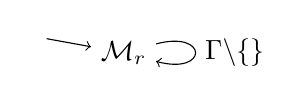
\begin{tikzpicture}
   \node (0) at (0,0) {$\M_r$};
   \node (init) at (-1.1,.2) {};
   \draw[->] (init) to (0);
   \draw[->,loop right] (0) to node {$\Gamma\backslash\{\blank\}$} (0);
  \end{tikzpicture}

  
  \item Linksmaschine $\M_L$
  
  Geht für beliebigen Bandinhalt nach links bis ein Blanksymbol erreicht ist und hält dann.

  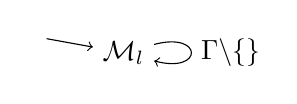
\begin{tikzpicture}
   \node (0) at (0,0) {$\M_l$};
   \node (init) at (-1.1,.2) {};
   \draw[->] (init) to (0);
   \draw[->,loop right] (0) to node {$\Gamma\backslash\{\blank\}$} (0);
  \end{tikzpicture}
 \end{itemize}
\end{Bsp}

Wir definieren das Flußdiagram und nun formal wie folgt.


\begin{Def}%[Flußdiagram]
Ein \emph{Flußdiagram} ist ein 7-Tupel $G=(\Sigma, \Gamma, \blank,V,E,v_0,L_V,L_E)$, dabei ist
\begin{itemize}
 \item $\Sigma$ ein Alphabet das wir \emph{Eingabealphabet} nennen,
 \item $\Gamma\supsetneq \Sigma$ ein Alphabet das wir \emph{gemeinsames Bandalphabet} nennen,
 \item $\blank\in \Gamma$ ein Zeichen, das wir \emph{gemeinsames Blanksymbol} nennen,
 \item $(V,E)$ ein gerichteter Graph,
 \item $v^\mathsf{init}\in V$ ein Knoten den wir \emph{Startknoten} nennen,
 \item $L_V$ eine Abbildung, die jedem Knoten eine Turingmaschine zuordnet und
 \item $L_E$ eine Abbildung, die jeder Kante $(v,v')\in E$ eine Teilmenge des Alphabets zuordnet.
\end{itemize}
\end{Def}


Notation: Bis zum Ende des Kapitels schreiben wir
$\M_v=\left(\Sigma,Q_v,\Gamma_v,\delta,\qinit,\blank,F_v\right)$
für die Turingmaschine $L_V(v)$, also die Turingmaschine die dem Knoten $v$ zugeordnet ist.

\begin{Def}%[Flußdiagram]
Die von einem Flußdiagram $G=(\Sigma, \Gamma, \blank,V,E,v^\mathsf{init},L_V,L_E)$ definierte Turingmaschine ist 
$\M=\left(\Sigma,Q,\Gamma,\delta,\qinit,\blank,F\right)$ wobei
\begin{itemize}
 \item $Q=\overset{.}{\bigcup\limits_{v\in V}} Q_v$
 \item $\qinit = \qinit_{v^\mathsf{init}}$
 \item $\delta(q,x) = 
 \begin{cases}
 (q',x',d) & \text{ falls } q\in Q_v \text{ und } (q',x',d)\in\delta_v(q,x)\\
 (q'',x,N) & \text{ falls } q\in Q_v \text{ und } \delta_v(q,x)=\{\} ...\\
 \{\} & \text{ sonst }
 \end{cases}$
 \item $F=\overset{.}{\bigcup\limits_{v\in V}} F_v$
\end{itemize}
\end{Def}

\subsection{Varianten von \ac{TM}s}

\begin{itemize}
	\item Endlicher Speicher\\
	Zum Abspeichern eines Elements aus endl. Menge $A$ verwende
	\[ Q'=Q\x A \]
	\item Mehrspurmachinen
	\begin{figure}[H]\centering
		{\renewcommand{\arraystretch}{0.8}
		\begin{tabu} to .5\textwidth {X[.35]|X[.65]}
			&\\\hline
			&\\\hline
			&\\\hline
			&\\\hline
			&
		\end{tabu}}
		\caption{Mehrspurmachine}
	\end{figure}
	
	Eine $k$-Spur \ac{TM} kann gleichzeitig $k\geq 1$ Symbole $\<- \Gamma$ unter dem Kopf lesen.\\
	Kann durch Standard \ac{TM} simuliert werden:
	\[ \Gamma' = \Sigma \overset{.}{\cup} \Gamma^k\text{ mit } \blank'=\blank^k \]
	\dots vereinfacht die Programmierung\\
	\begin{Bsp*}
		Schulalg. für binäre Addition, Multiplikation
	\end{Bsp*}
	\item \emph{Mehrbandmachinenen}\\
	Eine $k$-Band \ac{TM} besitzt $k\geq1$ Bänder und $k$ Köpfe, die bei jedem Schritt lesen, schreiben und sich unabhängig voneinander bewegen.
	\[ \delta_K:Q\x\Gamma^k \-> Q\x\Gamma^k\x \{R,L,N\}^k \]
	\item keine herkömmliche \ac{TM} (für $k>1$)
	\item kann durch $2k+1$ Spur \ac{TM} simuliert werden:\\
	\begin{tabular}{lll}
		Spur\\
		1 & \ruleplaceholder[ Band 1 ]{.5\linewidth}\\
		2 & \hspace{.23\linewidth}\# Kopf für Band 1\\
		3 & \ruleplaceholder[ Band 2 ]{.5\linewidth}\\
		4 & \multicolumn1r{\# Kopf\qquad\ }\\
		& \vdots\\
		$2k$ & \hspace{.09\linewidth}\dots\hspace{.09\linewidth} \# Kopf $k$\\
		$2k+1$ & \# &\#\#\\
		& linker Rand & rechter Rand
	\end{tabular}
\end{itemize}
\vspace{1em}

\begin{Satz}[name={[Simulation von $k$-Band \acs*{TM} durch 1-Band \acs*{TM}]}]
	Eine $k$-Band \ac{TM} kann durch eine 1-Band \ac{TM} simuliert werden.\quad $M=(Q\dots)$
\end{Satz}
\begin{proof}
	Zeige: ein Schritt der $k$-Band \ac{TM} wird durch endlich viele Schritte auf einer 1-Band \ac{TM} simuliert.
	\begin{enumerate}
		\item Schritt: Kodierung der Konfiguration der $k$-Band \ac{TM}\\
		Definiere $M'$ als \ac{TM} mit $2k+1$ Spuren und $\Gamma'=\Gamma\cup\{\#\}$
		\begin{itemize}
			\item Die Spuren $1,3,\dots,2k-1$ enthalten das entspr. Band von $M$: Band $i\<->$ Spur $2i-1$
			\item Die Spuren $2,4,\dots,2k$ sind leer bis auf eine Marke \#, die auf Spur $2i$ die Position des Kopfes auf Band $i$ markiert
			\item Spur $2k+1$ enthält\\
			\#\phantom{\#} Marke für linken Rand\\
			\#\# Marke für rechten Rand\\
			Zwischen den beiden Marken befindet sich der bearbeitete Bereich des Bands. D.h. die \ac{TM} arbeitet zwischen der linken und rechten Marke und schiebt die Marken bei Bedarf weiter.
		\end{itemize}
		
		\item Schritt: Herstellen der Start-Konfiguration.\\
		Annahme: Eingabe für $M$ auf Band 1\\
		Jetzt Eingabe (für $M'$) $w = a_1\dots a_n$
		\begin{enumerate}
			\item Kopiere $w$ auf Spur 1
			\item Kopf setzen auf Spur $2,\dots,2k$ an die Position des ersten Symbols von $w$
			\item auf Spur $2k+1$: \verb*!# ##!
	\end{enumerate}
	\begin{tabular}{*2{M{l}}}
		2k+1 & \#\blank\#\#\\
		2k & \#\\
		2k-1 & \blank\\
		\vdots\\
		4 & \#\\
		3 & \blank\\
		2 & \#\\
		\text{Spur }1 & a_1a_2\dots a_2
	\end{tabular} 
	
	Springe nach Sim($\qinit$), der Zustand in $M'$, an dem die Simulation des Zustands $q$ aus $M$ beginnt.
	
	\item Simulation eines Rechnerschritts im Zustand Sim($q$):\\
	Kopf auf linker Begrenzung, d.h. linker \# auf Spur $2k+1$
	\begin{itemize}
		\item Durchlauf bis rechter Rand, sammle dabei Symbole unter den Köpfen, speichern in endl. Zustand $\overrightarrow{\gamma} \in \Gamma^k$
		\item Berechne $\delta(q,\overrightarrow{\gamma})=(q',\overrightarrow{\gamma'},\overrightarrow{d})$\\
		neuer Zustand, für jeden Kopf ein neues Symbol $\overrightarrow{\gamma'}$ und Richtung $\overrightarrow{d}$.
		\item Rücklauf nach links, dabei Schreiben um $\overrightarrow{\gamma}'$ und Versetzen der Köpfe gem"a"s $\overrightarrow{d}$.
	\end{itemize}
	Falls eine Kopfbewegung den Rand auf Spur $2k+1$ überschreitet, dann verschiebe Randmarke entsprechend.
	
	Beim Rücklauf: Test auf Haltekonfiguration der $k$-Band \ac{TM}.\\
	Falls ja, dann Sprung in Haltekonf. von $M'$
	
	Weiter im Zustand Sim$(q')$.
	\end{enumerate}
\end{proof}

\begin{Korollar*}
	Beim Erkunden eines Worts der Länge $n$ benötige die $k$-Band Maschine $M\ T(n)$ Schritte und $S(n)$ Zellen auf den Bändern.
	\begin{itemize}
		\item $M'$ benötigt $O(S(n))$ Zellen
		\item $M'$ benötigt $O(S(n\cdot T(n)))$ Schritte $=O(T(n)^2)$
	\end{itemize}
	Weitere \ac{TM}-Booster
	\begin{itemize}
		\item Unbeschränkt großer Speicher
		\begin{itemize}[label=\->]
			\item für jede "`Variable"' ein neues Band
	\end{itemize}
	\item Datenstrukturen
	\begin{itemize}[label={\rotatebox[origin=c]{180}{$\Lsh$}}]
		\item ensprechend kodieren.
	\end{itemize}
	\end{itemize}
\end{Korollar*}

\subsection{Das Gesetz von Church-Turing (Churchsche These)} % 2.6
\begin{Satz}[name={[Intuitiv berechenbare Funktionen sind mit \acs*{TM} berechenbar]}]
	Jede intuitiv berechenbare Funktion ist mit \ac{TM} (in formalem Sinn) berechenbar.
	
	"`Intuitiv berechenbar"' $\equiv$ man kann Algorithmus hinschreiben
	\begin{itemize}
		\item endliche Beschreibung
		\item jeder Schritt effektiv durchführbar
		\item klare Vorschrift
	\end{itemize}
	Status wie Naturgesetz -- nicht beweisbar
	\begin{itemize}[label=\->]
		\item allgemein anerkannt
		\item weitere Versuche Berechenbarkeit zu formulieren, äquivalent zu \ac{TM}en erwiesen.
	\end{itemize}
\end{Satz}



\subsection{Universelle Turingmaschine}
Die bisher betrachteten Turingmaschinen waren (ebenso wie endliche Automaten oder Kellerautomaten) 
auf einen Einsatzzweck beschränkt und konnten nur eine bestimmte Sprache akzeptieren oder eine bestimmte Funktion berechnen.
Dies entspricht nicht unserer Vorstellung eines Computers, denn soch einer kann ja normalerweile beliebige Programme ausführen.

In diesem Kapitel konstruieren wir nun eine \ac{TM} $\M_U$ die als Eingabe sowohl
eine Codierung $\godel{\M}$ einer beliebigen \ac{TM} $\M$ als auch deren Eingabe $w$ nimmt, sodass die folgenden drei Eigenschaften gelten.
\begin{align}
	\label{Mu-eq-lang} w\in L(\M) &\Leftrightarrow \godel{\M}\#w) \in L(\M_U)\\ 
	\label{Mu-eq-term} \text{$\M$ terminiert bei Eingabe $w$} &\Leftrightarrow \text{$\M_U$ terminiert bei Eingabe $\godel{\M}\#w$}\\
	\label{Mu-eq-func} \text{$f_\M(w)$} &= \text{$f_{\M_U}(\godel{\M}\#w)$}
\end{align}

Wir nennen $\M_U$ die \emph{universelle Turingmaschine}.

\subsubsection{Codierung von Turingmaschinen}

Zunächst wollen wir uns eine Codierung $\godel{\M}$ für $\mathcal{\M}=(\Sigma, Q, \Gamma, \delta, \qinit, \blank, F)$ überlegen.
Die Effizienz unserer Codierung ist uns dabei nicht wichtig und wir versuchen der Einfachheit wegen mit Unärcodierungen zu arbeiten.

Einige Vorüberlegungen
\begin{itemize}
 \item Da $Q$ und $\Gamma$ endlich sind können wir jedem ihrer Elemente eine natürliche Zahl zuordnen.
 \item Wir müssen $\qinit$ und $\blank$ nicht explizit codieren, wir verwenden die Konvention, 
 dass $\qinit$ der Zustand mit der Nummer $1$ und $\blank$ das Zeichen mit der Nummer $1$ ist.
 \item Wir müssen $\Sigma$, $Q$ und $\Gamma$ nicht explizit in die Codierung mit aufnehmen.
 Für das Ausführen einer \ac{TM} sind nur die Elemente aus $\Sigma$, $Q$ und $\Gamma$ relevant die auch in der Transitionsfunktion $\delta$ vorkommen.
\end{itemize}

Idee: Codiere Elemente aus $Q$ und $\Gamma$ unär mit Hilfe von $0$ Zeichen.
Verwende $1$ Zeichen um unärcodierte Zahlen zu trennen.

\begin{itemize}
 \item Zustände
 
    Seien $q_1,\dots, q_{n}$ die Elemente von $Q$ sodass $q_1=\qinit$ 
    
    Definiere $\godel{q_i}:=0^i$
    
  \item Menge der akzeptierenden Zustände
  
    Seien $q_{k_1},\dots, q_{k_n}$ die Elemente von $F$
    
    Definiere $\godel{F}:=\godel{q_{k_1}} 1 \ldots 1 \godel{q_{k_n}}$
    
  \item Bandalphabet
  
    Seien $a_1,\dots, a_{n}$ die Elemente von $\Gamma$ sodass $a_1=\blank$
    
    Definiere $\godel{a_j}:=0^j$
    
  \item Richtung (in die der Schreib-Lesekopf bewegt wird)
  
    Definiere $\godel{L}:=0$, $\godel{N}:=00$ und $\godel{R}:=000$.
    
  \item Transitionsfunktion
  
   Seien $(q_{d_1}, a_{d_1}, q_{d_1}', a_{d_1}', r_{d_1}),\dots (q_{d_n}, a_{d_n}, q_{d_n}', a_{d_n}', r_{d_n})$ die Elemente von $\delta$.
  
   Definiere 
   
   $\godel{\delta}:= 11\godel{q_{d_1}}1\godel{a_{d_1}}1\godel{q_{d_1}'}1\godel{a_{d_1}'}1\godel{r_{d_1}}11\dots 11 \godel{q_{d_n}}1\godel{a_{d_n}}1\godel{q_{d_n}'}1 \godel{a_{d_n}'}1\godel{r_{d_n}}11$
   
   \item Turingmaschine
   
   $\godel{\M}:=111\godel{\delta}111\godel{F}111$
\end{itemize}


\subsubsection{Arbeitsweise der universellen Turingmaschine}
Da die universelle Turingmaschine $\M_U$ recht komplex ist wollen wir diese hier nicht formal definieren sondern geben nur eine informelle Beschreibung der Arbeitsweise.


Wie definiere $\M_U$ als 3-Band Maschine wobei die Bänder $B_1$, $B_2$ und $B_3$ wie folgt genutzt werden.
\begin{itemize}
\item[$B_1:$] Zu Beginn steht hier die Eingabe für $\M_U$.
Nach der Initialisierung von $\M_U$ verwenden wir $B_1$ um das Band der Eingabeturingmaschine $\M$ nachzuahmen.
\item[$B_2:$] Speichere die Codierung der Eingabeturingmaschine $\ulcorner \M \urcorner$
\item[$B_3:$] Speichere den aktuellen Zustand von $\M$ ($0^k$ für Zustand $q_k$)
\end{itemize}

Die universelle Turingmaschine $\M_U$ beginnt zunächst mit einer Initialisierung die aus den folgenden drei Schritten besteht.

\begin{enumerate}
 \item Prüfe ob der erste Teil der Eingabe $\ulcorner \M \urcorner$ eine gültige Turingmaschine codiert.
 
 Die Menge der gültigen Codierungen kann mit Hilfe einer kontextfreien Grammatik beschrieben werden (siehe Übungen).
 
 \item Verschiebe $\ulcorner \M \urcorner$ auf $B_2$. Schreibe dabei Blanksymbole auf die Bandzellen von $B_1$.
 Überschreibe anschließend das Symbol $\#$ das Eingabeturingmaschine und Eingabewort trennt durch ein Blanksymbole.
 
 \item Schreibe $0$ (also die Codierung des Startzustandes von $\M$) auf $B_3$.
\end{enumerate}

Nach der Initialisierung ist $\M_U$ also in der folgenden Konfiguration.
\begin{itemize}
\item[$B_1:$] $w$
\item[$B_2:$] $\ulcorner M_0 \urcorner$
\item[$B_3:$] $0' \sim Z,q$
\end{itemize}

Nach der Initialisierung wird $\M_U$ das Verhalten von $\M$ nachahmen.
Für jeden Schritt von $\M$ macht $\M_U$ dabei die folgenden Schritte.

 Suche ein Element $(q, a, q', a', r)$ der Transitionsfunktion $\delta$ von $\M$ das zum aktuellen Zustand $q$ und zum aktuellen Eingabesymbol $a$ passt.
 
 Wir laufen hierfür einmal über das komplette Band $B_2$. 
 Zustände werden Zeichenweise mit dem Inhalt von $B_3$ verglichen.
 Die Zuordnung von Alphabetsymbolen zu codierung ist fest in $\M_U$ eingebaut.
 
 \begin{itemize}
 
 \item Falls es solch ein Element der Transitionsfunktion existiert,
    schreibe auf $B_1$ das Zeichen $a'$ und Bewege den Kopf wie durch $r$ definiert.
    Ersetze außerdem die Codierung $\godel{q}$ auf $B_3$ durch $\godel{q'}$.
    Fahre anschließend mit dem Nachahmen des nächsten Schrittes von $\M$ fort.
    
 \item Falls kein solches Element der Transitionsfunktion existiert hat $\M$ eine Haltekonfiguration erreicht.
 Wir vergleichen nun den aktuellen Zustand (auf $B_3$) mit den auf $B_2$ gespeicherten akzeptierenden Zuständen und akzeptieren oder verwerfen die Eingabe entsprechend.

\end{itemize}

\begin{Satz}
	Die universelle \ac{TM} $\M_U$ erfüllt die Eigenschaften (\ref{Mu-eq-lang}), (\ref{Mu-eq-term}) und (\ref{Mu-eq-func}).
\end{Satz}


%%% Local Variables:
%%% mode: latex
%%% TeX-master: "Info_3_Skript_WS2016-17"
%%% End:
